\chapter{The Yakkha language and its speakers}\label{languageintro}
\todo{Please use only exhaustive sections; See Generic Style Rules pg 2}
This chapter provides basic information on the geographic (\sectref{geogr}) and cultural-historical  background of the Yakkha language (\sectref{cult-hist}), a genealogical classification of Yakkha as a member of the Kiranti language family (\sectref{genetic}), and its sociolinguistic (\sectref{socioling}) context. The reader should note that the  following observations are not made by a trained anthropologist. An in-depth anthropological study is beyond the scope of this introductory chapter (see \sectref{earlier-work} for existing anthropological studies). 

In this chapter, the term  Kiranti can indicate both ethnic and linguistic affiliations. It refers to a group of roughly 30 ethnically and linguistically distinct, yet related, communities in eastern Nepal. The internal structure of the Kiranti group is complex, and linguistic classifications may deviate from ethnic classifications, cf. \sectref{cult-hist} below.

\section{Geographical context}\label{geogr}

Nepal can roughly be divided into three geographical zones: the Himalayan range in the north, the middle hills (the Mahabharat range, stretching parallel to the Himalayan range) and the plains in the south (the Tarai). The Himalayan range is home to speakers of Tibeto-Burman languages. The plains are mostly inhabited by speakers of Indo-Aryan languages. Furthermore, a few Austroasiatic languages, one Dravidian language and an isolate (Kusunda) are spoken in Nepal. Speakers of Kiranti languages, including Yakkha (see \figref{nepalmap}), inhabit the hilly area between the Likhu river in the west and the border with Sikkim in the east, with elevations between 1,500m and 2,700m. Kiranti  settlements can also be found in the plains and in India (Darjeeling, Sikkim). 

\begin{figure}
\centering
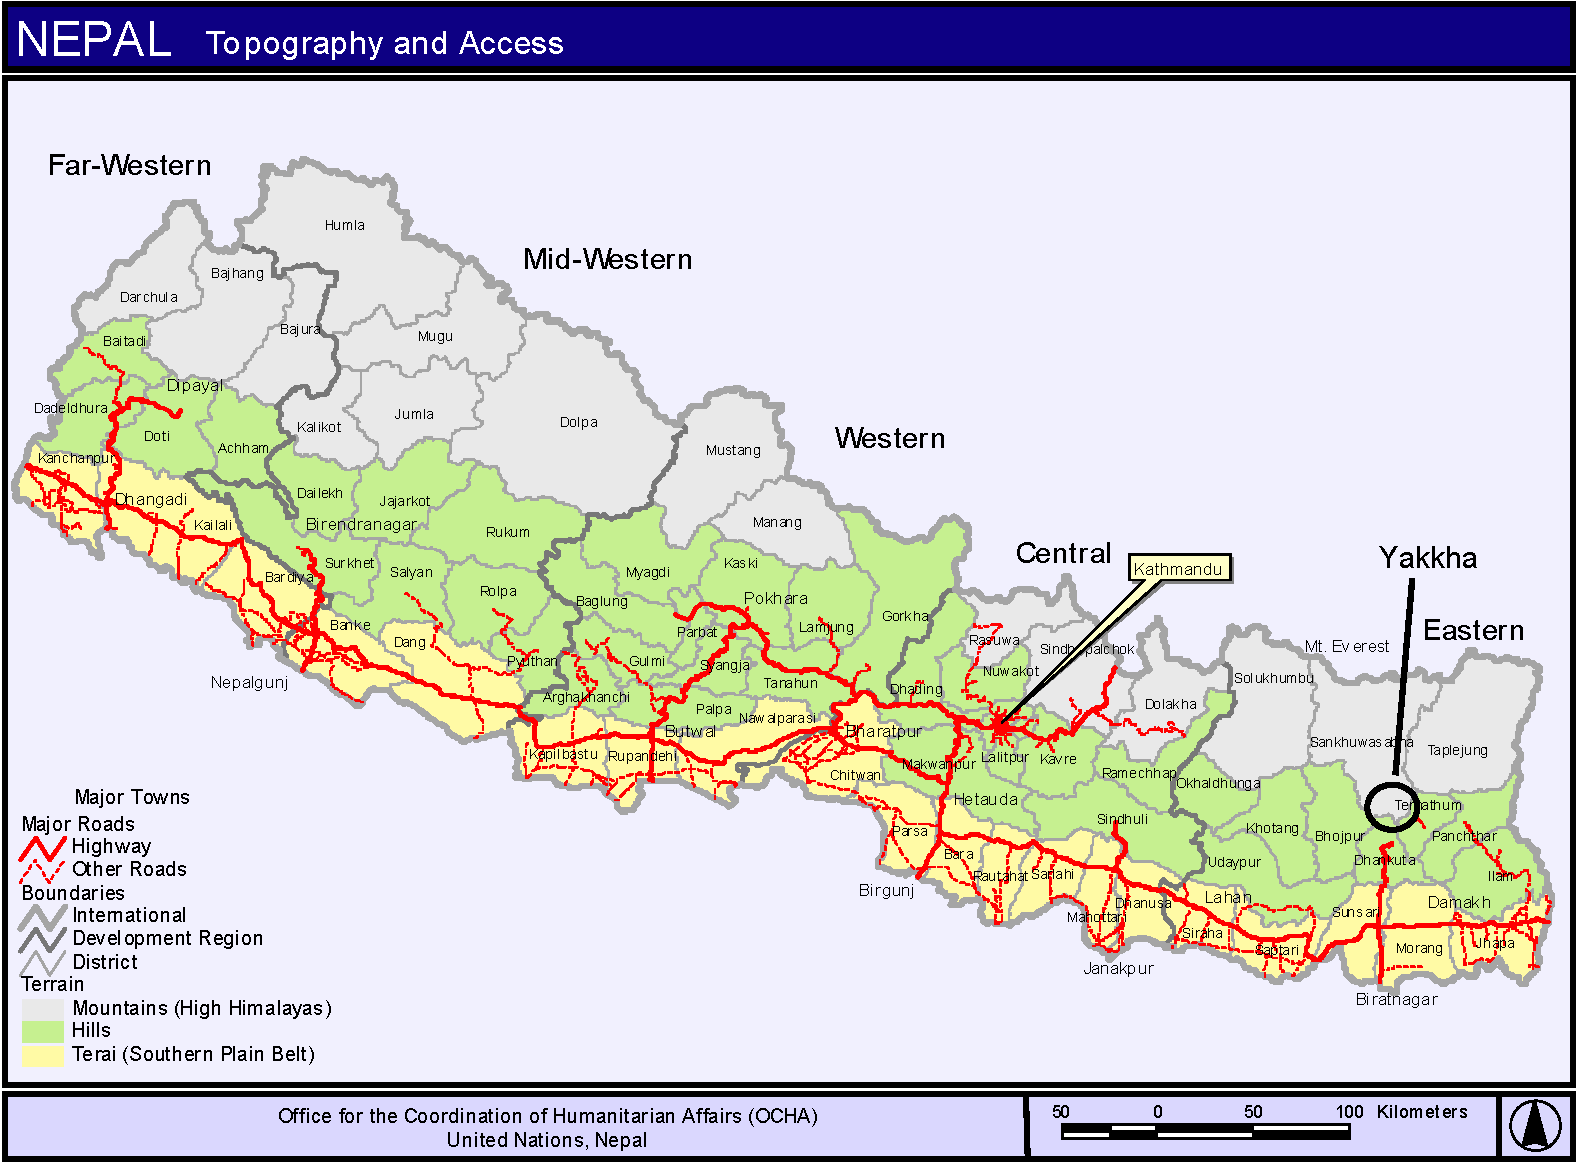
\includegraphics[width=11cm]{figures/Nepalkarte.pdf}
\caption{Location of the Yakkha region within Nepal (United Nations Map Centre: http://www.un.org.np/resources/maps, accessed on 17 January 2014 )}\label{nepalmap}
\end{figure}

The Yakkha region (i.e. the area inhabited by people who consider themselves Yakkha ethnically)\footnote{If the region were defined by linguistic criteria, it would be much smaller; see \sectref{endangerment}.} is located in the Koshi zone of the Eastern Development Region, in the south of Sankhuwa Sabha district and in the north of Dhankuta  district  (see the maps in \figref{map-sank} and \figref{map-dhan}). Within the region in  Eastern Nepal commonly known as \emph{Kirant} (\rede{Kiranti area}), the Yakkha region belongs to the \emph{Pallo Kirant} \rede{Far Kiranti area}, located on the east of the Arun river. 

The core Yakkha region contains the following Village Development Commitees (\textsc{vdc}s):\footnote{Nepal is administratively divided into 5 development regions, 14 zones, 75 districts and  3,913 village development commitees (\textsc{vdc}s). Each \textsc{vdc}  contains several villages and is further divided into numbered wards.} Canuwa, Marek Katahare and Dandagaun in Dhankuta district, and Tamaphok (Tamfok in the map), Mamling, Ankhinbhuin, Madi Mulkharka, Madi Rambeni, Baneshwor, Chainpur, Kharang, Wana (Bana in the map), Siddhakali, Siddhapokhari and Syabun in Sankhuwa Sabha district. The Yakkha region is also known as the \emph{Tin Thum} (\rede{The Three Regions}): the \emph{Das Majhiya} in the south, the \emph{Panch Majhiya} in the middle and the \emph{Panch Kapan} in the north  \citep[86]{Kongren2007Indigenous}, a distinction originating in the tax system that was enforced under the Gorkha rule in the 18\textsuperscript{th} century. The language is  only spoken by parts of the Yakkha population, being replaced by Nepali in almost half of the geographic area inhabited by Yakkha people. Curiously, the language proficiency decreases drastically towards the north of the Yakkha area (Magman Linkha, p.c.), contrary to the expectation that greater distance to the main roads and thus greater isolation should have had a positive effect on the preservation of a language. 



\begin{figure}
\centering
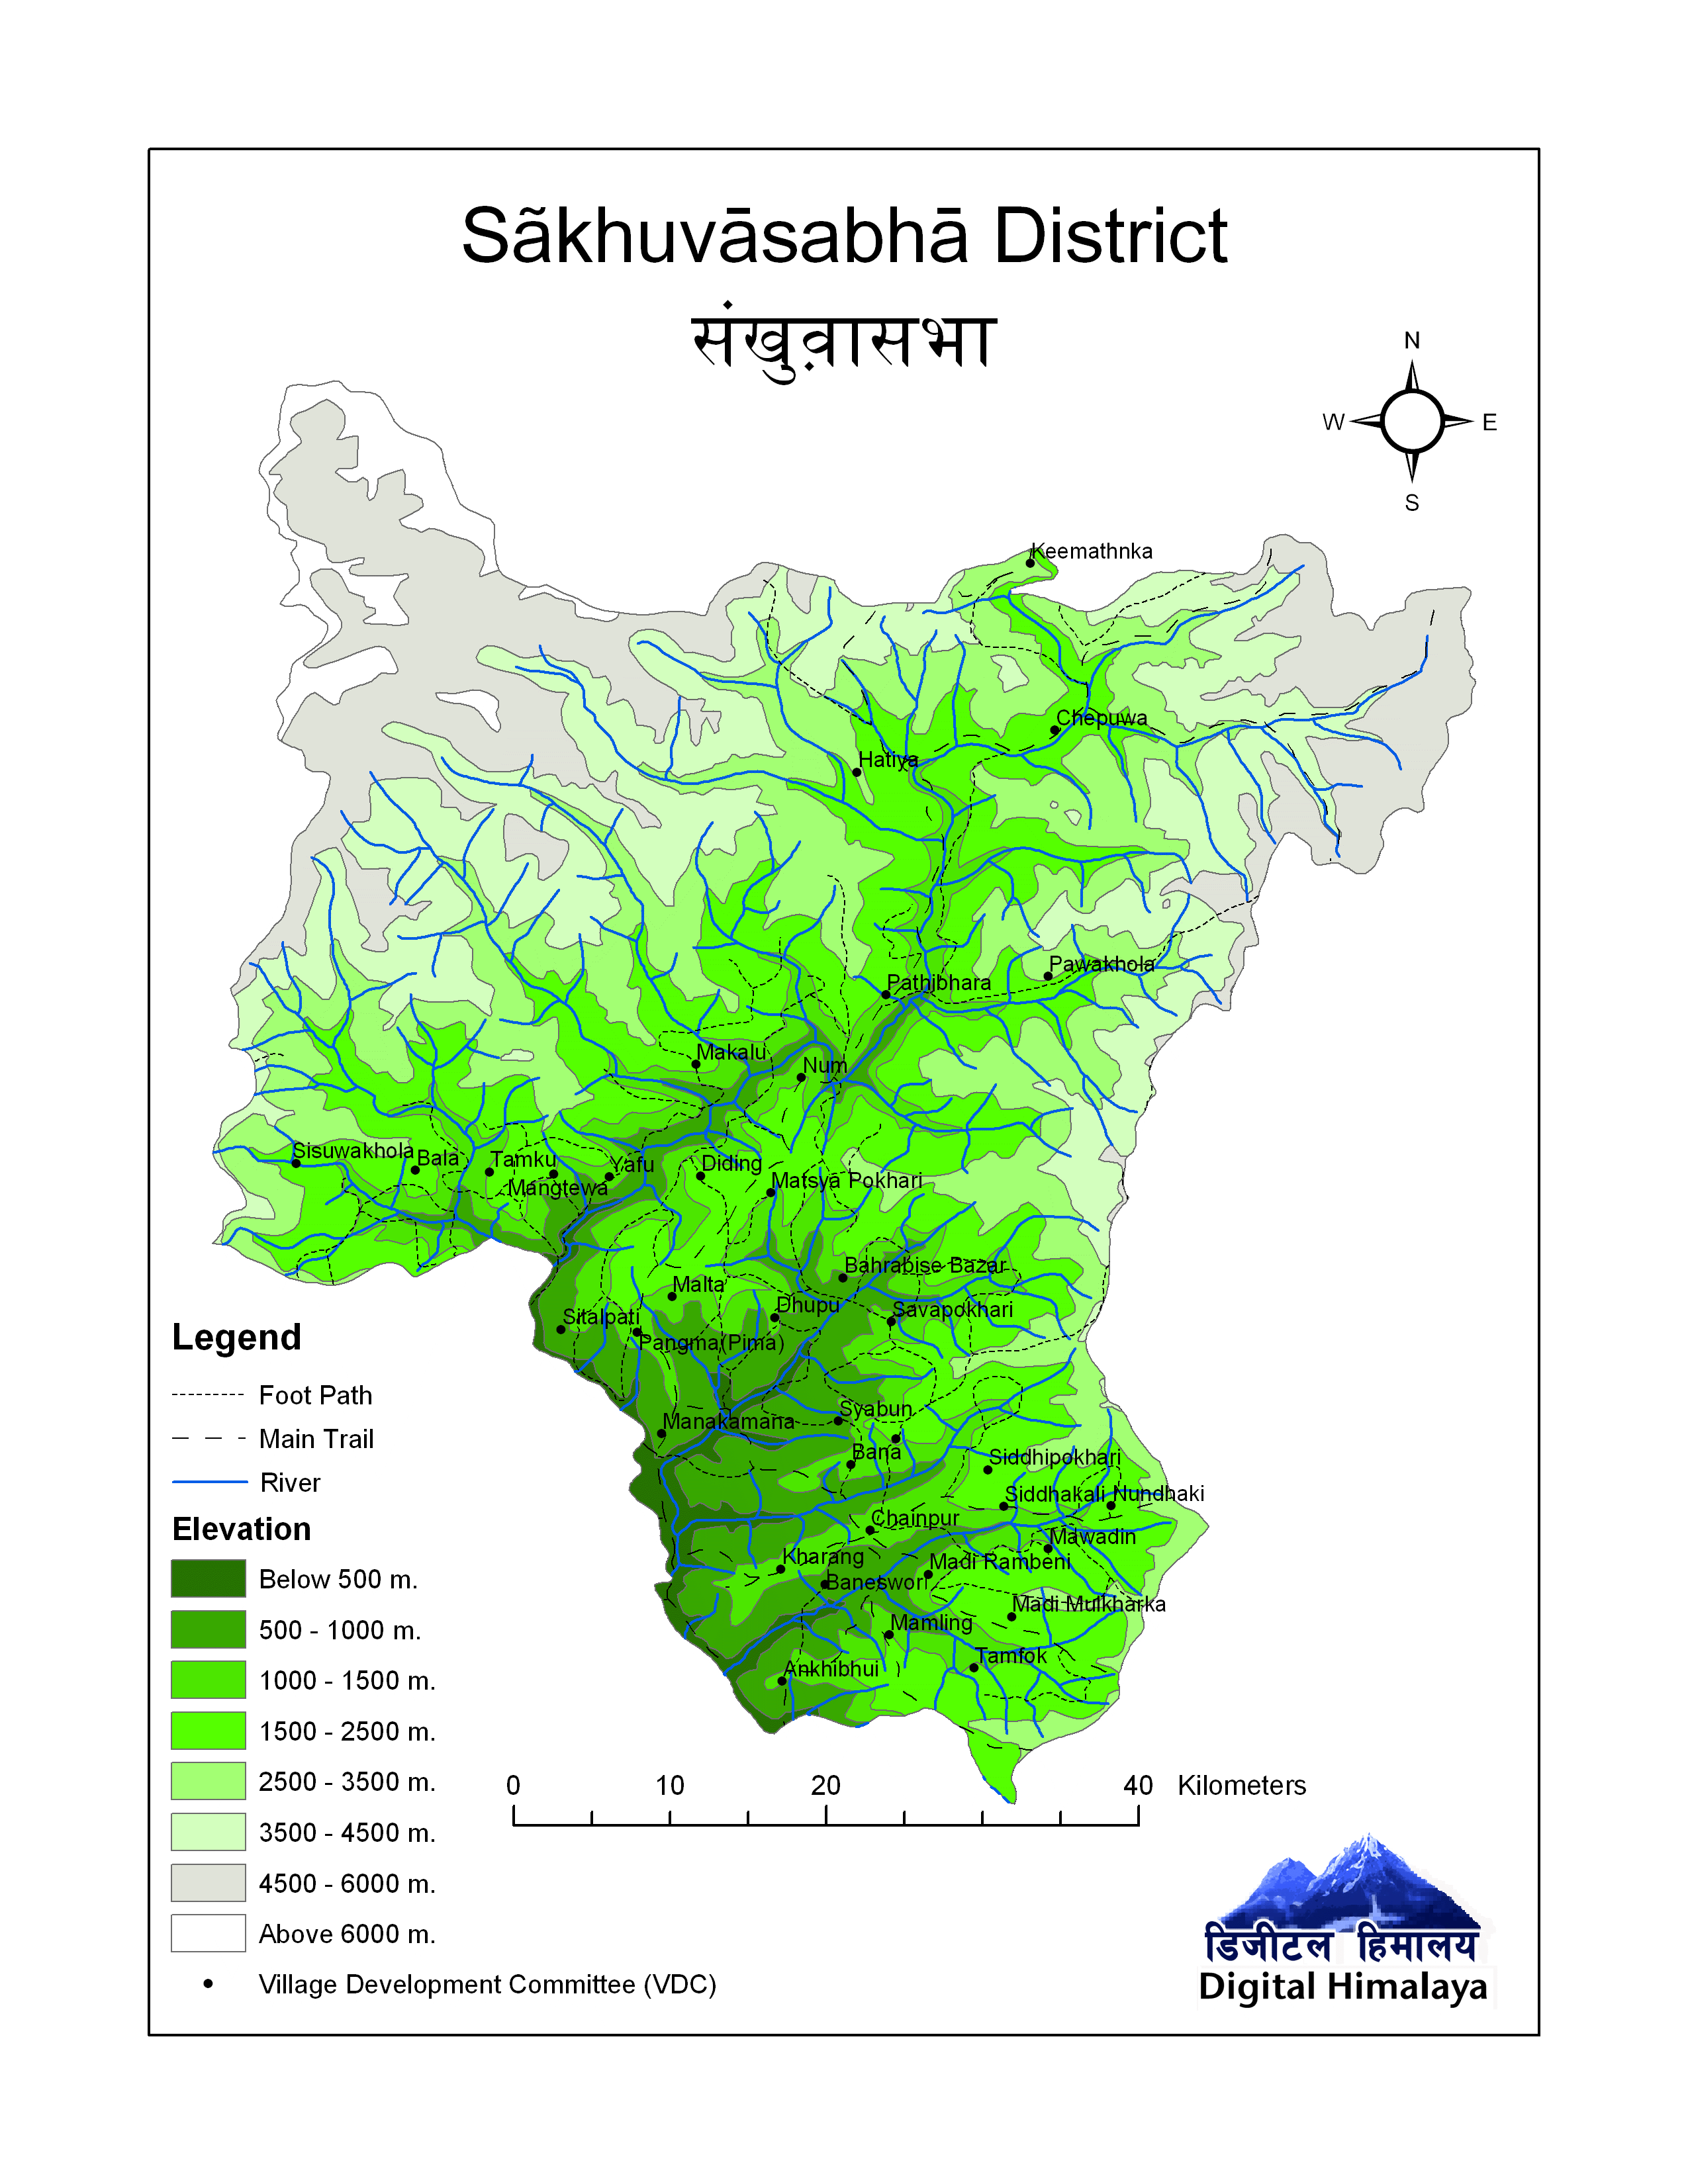
\includegraphics[height=15cm]{figures/district_sankhuwasabha_everything.png}
\caption{Map of Sankhuwa Sabha district, with Yakkha villages in the south \citep{Joshi_Nepal_maps}}\label{map-sank}
\end{figure}

\begin{figure}
\centering
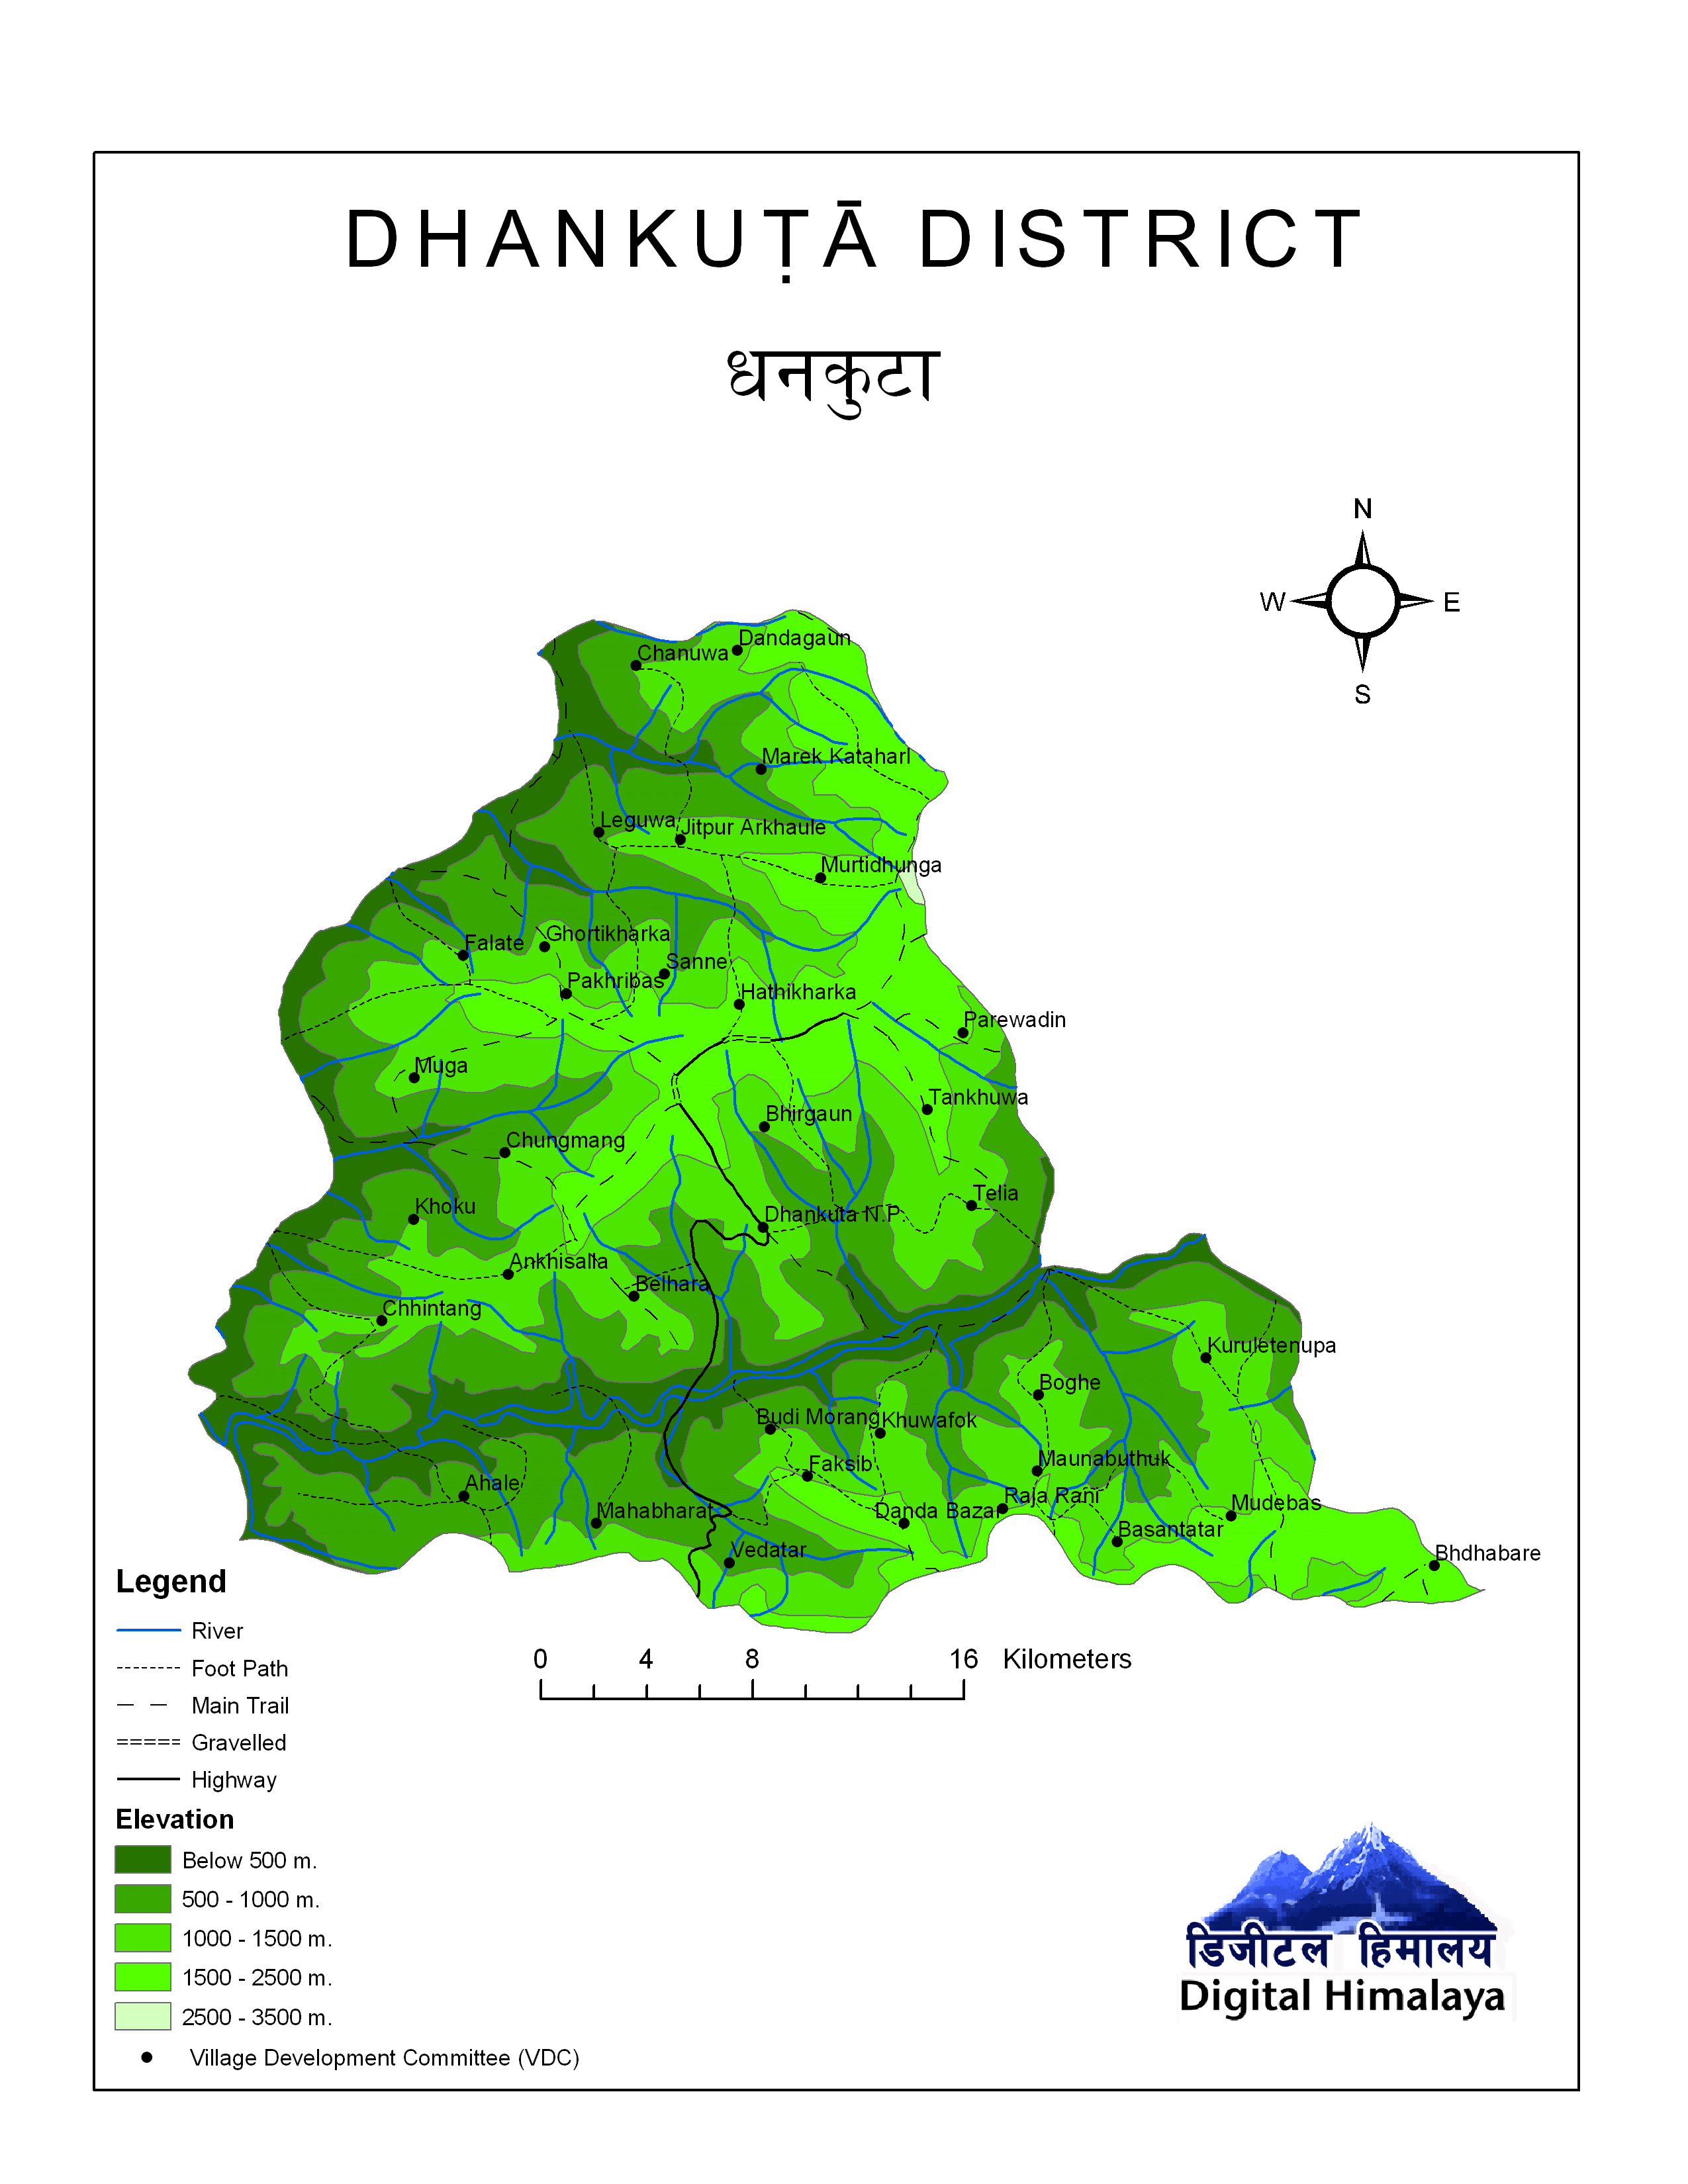
\includegraphics[height=15cm]{figures/district_dhankuta_everything.png}
\caption{Map of Dhankuta district, with Yakkha villages in the north \citep{Joshi_Nepal_maps}}\label{map-dhan}
\end{figure}

Yakkha has at least four dialects (see \sectref{sc-dialect} below). The focus of this work is on the Tumok dialect, named after the village where it is spoken (27.208°N, 87.384°E), in Tamaphok \textsc{vdc}.\footnote{Tamaphok is also the Nepali name of Tumok. Many Yakkha villages have both a Nepali name and a Yakkha name. Impressionistically, Yakkha names are used to refer to particular villages, while  Nepali names are used to refer  to \textsc{vdc}s (which are in general conglomerations of several villages). This is also the case e.g. for Waleng (Nepali: \emph{Madi Mulkharka}), Yaiten (Nepali: \emph{Dandagaun}) and Angbura (Nepali: \emph{Omruwa}).} Tumok  lies on the south-western slopes of the Maya Khola valley.\footnote{\emph{kholā} is a Nepali word for \rede{little river}.} The Maya Khola flows north-west into the Piluwa Khola, which is a tributary of the Arun river (the main river in the region, partly flowing along the south-western border of Sankhuwa Sabha district). Tumok  is located approximately 1500m above sea level. Villages in this hilly region generally spread over several hundred meters of altitude, because the houses are not built close to each other, allowing space for fields between them. The great extension of the villages may lead to climatic differences and to differences in the crop cycle even within one village. The speaker density in Tumok is very high, and even parts of the non-Yakkha population speak Yakkha in addition to Nepali.\footnote{Among the non-Yakkha population, it is more common to speak Yakkha for members of castes that were perceived as “low” (according to Hindu social law)  than for members of so-called “high” castes. Despite changes in the legal system, these distinctions still play a role in social practice and thus, it is more attractive for members of discriminated groups to learn Yakkha, while members of “high” castes often do not know any Yakkha, even after having lived in the area for decades.} \figref{tumok} shows the view from Tumok towards the Himalayan range in the north. 

\begin{figure}
\centering
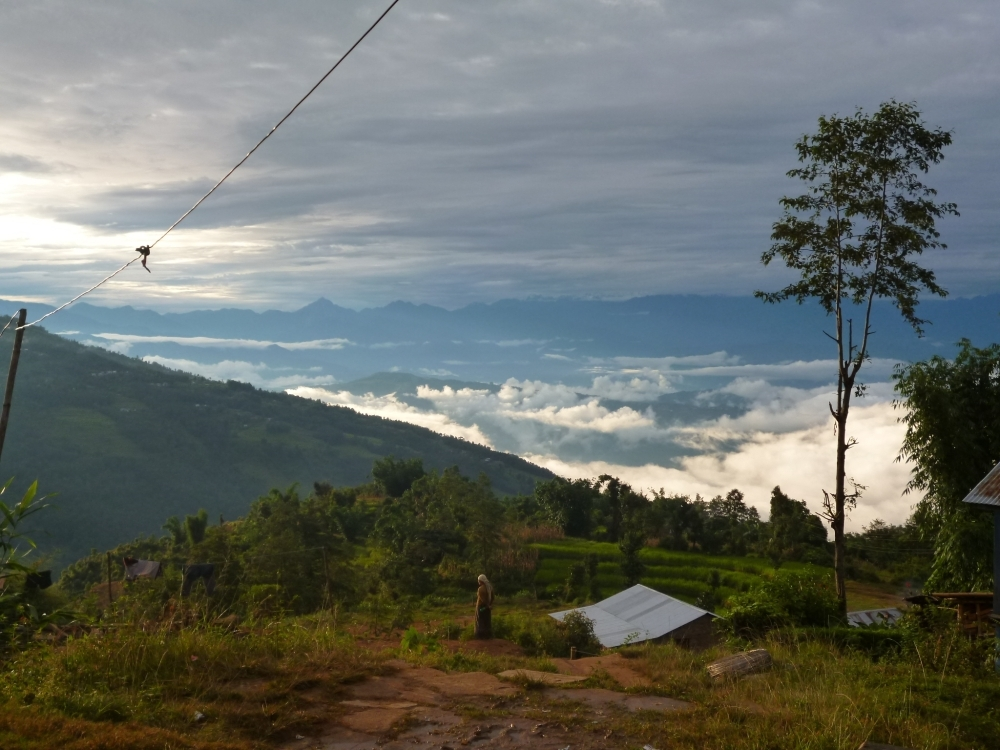
\includegraphics[width=10cm]{figures/tamaphok.jpg}
\caption{Tumok at the end of the rainy season, Sept. 2012}\label{tumok}
\end{figure}
 

Yakkha speakers can also be found outside the core area defined above. There are about 80 households in the south-east of Dhankuta district, in Mudhebas \textsc{vdc}, Kuruletenupa \textsc{vdc} and Bodhe \textsc{vdc} (Magman Linkha, p.c.). In Ilam district, a Limbu-speaking region bordering with India, Yakkha speakers are reported to live in Namsaling village, speaking a dialect that is perfectly intelligible with the Yakkha from the core area. Nowadays there are also many Yakkha people living outside the hills, in the city of Dharan (Sunsari district) and other places in the Tarai and in India (especially in Darjeeling and Sikkim). A common reason for migration is the search for land or employment. Of course, Yakkha are also found elsewhere in the world due to the high rate of Nepali emigration for the previously mentioned reasons as well as education. 

The Yakkha region is surrounded by other Kiranti languages. Going clockwise, starting in the east, these are Limbu (including the Tamarkhole, Phedappe  and Chatthare dialects). Athpare,  Chɨlɨng, Belhare and Chintang follow in the south, Bantawa and Dungmali in the west, Mewahang, Lohorung and Yamphu in the north. This geographical classification has to be understood in an idealized sense. Most of the villages in Nepal are ethnically and linguistically diverse, so that one may also find Sherpa, Gurung, Tamang, Newari and Parbatiya (Nepali speaking) households in the Yakkha region.

  

\section{Cultural and historical background}\label{cult-hist}

\subsection{Kiranti}


Kiranti (also Kirāt, Kirāta, Kirā̃ti) nowadays refers to a set of roughly 30 communities speaking related languages, who inhabit the Himalayan foothills in Eastern Nepal and share key cultural practices, including nature worship and a body of oral knowledge, myth and ritual in which the veneration of ancestors plays a major role (known as \emph{Munthum} in Yakkha). Within these parameters, however, there is considerable heterogeneity of cultural practices, beliefs and origin myths, and shifting ethnic and linguistic affinities do not seem to be uncommon (Yakkha itself being a prime example, as will be explained further below).\footnote{Although this is commonly overlooked in current politics in Nepal,  present-day ethnic distinctions are the product of several waves of migrations and millenia of mutual influence in the Himalayan contact zone of Indosphere and Sinosphere (terms from Matisoff, e.g. \citealt{Matisoff1990_On}). The perception of distinct “pure” and time-stable ethnic and linguistic groups presents a highly idealized picture that does not do justice to the complex social reality of a multi-ethnic country like Nepal. Most current ethnic identities have been shaped by mixing with other groups or by adapting to other groups in one way or another, and these processes are, of course, continuing in the present.} 

We have very little historically verified knowledge about the Kiranti people.\footnote{The work of renowned Limbu historiographer Iman Singh \citet{Chemjong1967History}, widely perceived as the major source on Kiranti history among the Kiranti people, uses the available sources (both western scholarly work and indigenous chronicles) with few epistemological criticisms, and does not provide sufficient evidence to be called historical in the academic sense. It is rather to be seen as an attempt to anchor Kiranti culture in the deepest past possible and the widest  area possible, with  evidence spanning large parts of Eurasia from Greece to Cambodia \citep[125]{Schlemmer2003_New}. Despite its methodological shortcomings, Chemjong's work must be praised for its contribution to the acknowledgement and recognition of a distinct and unique Kiranti culture (see also \citealt[340]{Gaenszle2002_Remaking}).} The term Kiranti comes from Sanskrit \emph{kirāta} and dates back to Vedic texts such as the Atharvaveda, which is considered the oldest Veda after the   R̥gveda \citep[594]{Driem2001Languages}. It is generally accepted by Nepali and foreign historians alike that kings known as Kiranti (or Kirāta) must have ruled over central Nepal before they were overthrown by the Lichhavis early in the first millenium CE \citep[13]{Whelpton2005A-History}.  However, the well-documented history of Nepal unfortunately only begins with the Lichhavi dynasty, so that it is not at all clear whether the ancient Kirantis were the forefathers of the Kiranti people who currently live in eastern Nepal. One should note that in  the old Indian texts the term \emph{kirāta} had a much broader reference, applying to Tibeto-Burman hill peoples in general \citep{Whelpton2005A-History, Schlemmer2003_New}. The self-designation Kiranti in the present sense came to be used only with the advent of the Gorkha kings, when a common Kiranti identity began to evolve under Hindu dominance \citep[340]{Gaenszle2002_Remaking}. Before that era, there was no common feeling of being Kiranti: clan affinities were most important, and autonyms such as Khambu/Khombo (for the Rai) and Yakthumba (for the Limbu) were used among the Kiranti groups.


Present-day Kiranti legends trace the groups' origins to a variety of locales, from Tsang in Tibet to Varanasi in the Gangetic plains (see \citealt[xix]{Driem1987A-grammar} for Limbu), or places in the Tarai (see \citealt[34]{Gaenszle2012_Where} for Mewahang).\footnote{The Yakkha legends I recorded are about their ancestors' deeds and journeys in the area where present-day Yakkha people live. My own materials do not contain myths regarding a prior place of origin. This does not imply that there are no such myths. I have recorded only eight narratives, which is probably not even close to representative of what is still out there, unrecorded. In general, the Kiranti groups have a strong concern for the past and vibrant oral traditions in which origins and migrations are recalled for many generations \citep{Gaenszle2000Origins, Gaenszle2002_Remaking}.} It is not known when and how the ancestors of the Kiranti groups entered Nepal, but it is very likely that they came at least 2000 years ago from the east \citep{Driem2001Languages, LaPolla2001_Role, Gaenszle2002_Remaking}. Kiranti languages show striking similarities with rGyalrongic languages spoken in the South of China and with the extinct Tangut language, especially with regard to hierarchical patterns in the person marking system (see e.g. \citet{DeLancey1981_Category, Ebert1990Evidence, LaPolla2007Hierarchical, Jacques2012_Agreement}, and also \sectref{verb-infl} and \sectref{obl} of this work), although direct contact between these  groups has not been proven.\footnote{There is a scholarly debate as to whether these similarities are Proto-Tibeto-Burman (and got lost in the other languages) or whether the groups showing hierarchical patterns in person marking form a separate branch of Tibeto-Burman (see e.g. \citealt{Driem1991Tangut, LaPolla2001_Role, DeLancey2010_Towards, Jacques2012_Agreement, LaPolla2012_Comments}). The debate boils down to the still unsettled question of whether Proto-Tibeto-Burman had person marking morphology or not, and it will probably only be settled once more data on Tibeto-Burman languages are available.} Another argument for  migration from the east is that those Tibeto-Burman groups that have entered Nepal via the north, such as the Tamangs for instance, show a close relation to Tibetan culture and Tibetan Buddhism \citep{LaPolla2001_Role}, while Kiranti culture is clearly distinct from Tibetan culture.\footnote{To provide a culinary example: fermented soybeans (\emph{kinama} in Yakkha) are an integral part of the Kiranti cuisine. While this dish is not widely cherished outside the Kiranti sphere in Nepal, it is widespread in Northeast India (e.g. in Nagaland), and  also known from Thailand, Burma, Korea and Japan \citep{Tamang2010_fermented}.} 
%in Jacques: Baumann 1975, DeLancey 1981, van Driem 1993, Ebert 1990
 
The Kiranti peoples' more recent history has been described in various sources  \citep{Caplan1970_Land, Pradhan1991The-Gorkha, Gaenszle2002_Remaking, Schlemmer2003_New, Whelpton2005A-History} and will  only be briefly summarized here. As a nation state, Nepal was founded by Pr̥thvī Nārāyaṇ Śāha (1723--1775), the king from Gorkha\footnote{Gorkha is a district in the Western Development Region of Nepal.} who conquered the area known as Nepal today. Seen as a hero by Nepali nationalists, for the ethnic minorities his name stands for the suppression of their cultures and languages. Local groups confronted the king and his successors with strong armed resistance, but eventually Gorkha rule was established. The Kiranti region, bordering British-ruled Sikkim in the East, was critical to maintaining the Gorkha rule, and in order to keep the Kiranti groups loyal, they were given a privileged status and a certain degree of autonomy. In a system known as \emph{kipāt}, land rights were reserved for Kiranti people who owned the land by virtue of their ethnic affiliation. Local headmen were appointed to collect taxes. The titles given to them (Rai, Subba, Jimdar) are still reflected in contemporary Kiranti surnames. Later, the Gorkha kings changed their strategy and sought to control and assimilate the Kiranti region. Kiranti groups were officially incorporated into the caste system (as \emph{matvāli jāt}, \rede{drinking caste}), and the state encouraged Hindu settlers to move east. They were allowed to take control of land previously held by Kiranti people, thus systematically undermining the \emph{kipāt} system. Brahmanic values became more influential, Nepali was propagated as the national language and attempts to express and preserve one's ethnic identity were suppressed as threats to the nation state. On an everyday level,  obviously some expression of \rede{Kiranti-ness} must have continued, because distinct Kiranti cultural practices are still present nowadays (see also the observations made by \citealt{Russell2004Traditions}).
 
Hindu dominance began to erode only recently, with the 1990 constitution, in which Nepal's multi-ethnic and multi-lingual social reality was officially acknowledged for the first time (Article 4), and more so since the end of the monarchy in 2006. Currently, a new and strong sense of a common Kiranti identity is emerging, which can be attributed to the recent climate of rising ethnic consciousness (over the last two decades). The different Kiranti groups (Limbu, Rai, Yakkha, Sunwar) now share a newly-built temple in Sāno Hāttiban in the south of Kathmandu and they celebrate festivals together that were originally celebrated separately, on
village level.\footnote{Cf. \citet{Gaenszle_Redefining} on the changes that Kiranti culture and religion are currently undergoing now that more and more people live outside the rural homeland.}  The mythical king Yalambar has undergone a revival as the legendary founder of the Kiranti dynasty, an iconic figure representing an idealized glorious past. A recently built and newly-renovated statue of Yalambar in the market town Mudhe Sanischare in Sankhuwa Sabha district may illustrate the perspective that Kiranti people themselves have on their origins (see \figref{yalambar}).\footnote{See e.g. \citet{Schlemmer2003_New} for a critical assessment of the re-invention of the Kiranti past that came along with the ethnic revival in contemporary Nepal, in particular the widespread booklets and online publications that construct an ancient and glorious Kiranti past that is not grounded in historical evidence. Schlemmer notes that such a re-invention of history often originates from a mostly urban middle class that is disconnected from its rural homeland. According to my own observations, with the number of educated people rising in the villages, with roads being built and more people regularly commuting between cities and their villages, ethnic self-awareness is increasing also in the rural areas.}

\begin{figure}
\centering
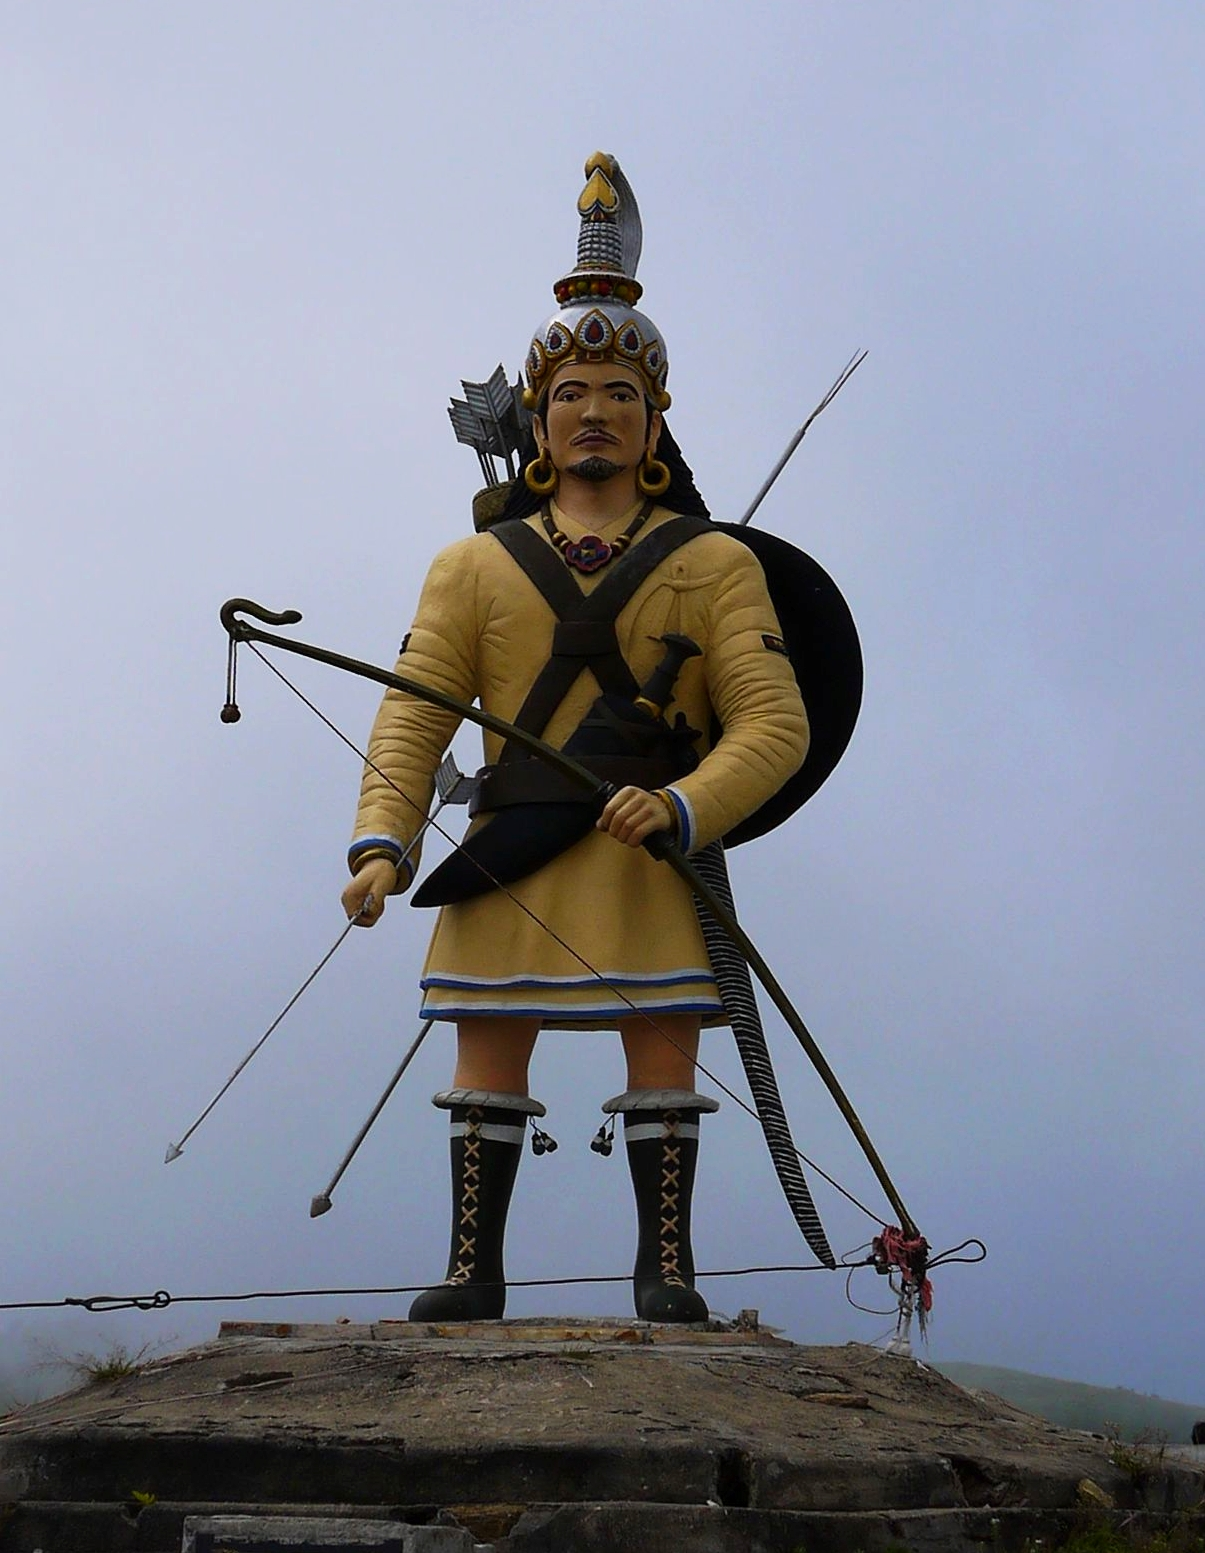
\includegraphics[height=8cm]{figures/yalambar.jpg}
\caption{The statue of the mythical Kiranti king Yalambar in Mudhe Sanischare}\label{yalambar}
\end{figure}


Another iconic figure for Kiranti identity is the 18\textsuperscript{th}-century Limbu scholar Te-ongsi Sirijunga Xin Thebe (Sirijanga) from Sikkim, who is celebrated as the initiator of an ethnic awakening and as the creator of the Limbu script (legendary accounts state that he found and revived the script). He is widely perceived as a martyr for the Kiranti cause, because he was  murdered by the Sikkimese Bhutia rulers, allegedly because they perceived his activities as a threat. He is usually depicted tied to a tree and bristling with arrows, for instance in a statue in Dharan (Tinkune), but also in icon-like prints and posters that can be found in people's homes.


\subsection{The Yakkha}

\subsubsection{Ethnic affiliation}

Within Kiranti, the largest subgroups are the Rai and the Limbu. While the Limbu speak a few very closely related languages, the term Rai is a broad category that subsumes at least 20 linguistically and ethnically distinct communities.  

The Yakkha perceive themselves as closest to the Limbu both culturally and linguistically (see also \citet[90]{Russell1992_Yakha}). Marriages between Yakkha and Limbu are more common than between members of other Kiranti groups. The closest linguistic relative of Yakkha, however, is not Limbu, but the Belhare language, since Yakkha and Belhare share some innovations and unique features that are not found in any other Kiranti language (cf. \sectref{genetic} below). The most likely historical scenario is that the Yakkha have adapted culturally to the Limbu because the latter have been  the economically and socially most powerful group in the region. 

Formerly, the Yakkha were also known as Rai \citep[90]{Russell1992_Yakha}.\footnote{Russell suggests that the name Rai was used when communicating with outsiders to benefit from the reputation of those Rai in the British Gurkha regiments. In present times, too, when talking about my research outside the Yakkha area, I was frequently confronted with the assumption that the Yakkha are a Rai group.}  The Yakkha, however, stress that they neither belong to Rai nor to Limbu. In line with this, it is now popular to use \emph{Yakkha} or one's  clan name as surnames instead of the formerly used exonymic surnames \emph{Dewan} and \emph{Jimi} that originate in Nepali administrative titles given to local tax collectors by the Gorkha kings.\footnote{Cf. \citet[8]{Doornenbal2009A-grammar} for the same observation in Bantawa.} Furthermore,  origin myths that are known from many Rai groups, such as the story about Sumnima and Paruhang or the legends about the orphan hero Khocilipa/Khakculukpa \citep{Ebert2003Camling, Gaenszle2000Origins} are not perceived as native to Yakkha and are not widely known. 

The nature of the historical link to Belhare, which is spoken near Dhankuta, 50 kilometers to the  south of the core Yakkha area, is not known with certainty, but it is worth noting that \citet[13, 47]{Dahal1985An-ethnographic}\footnote{Cited in \citet[1]{Russell1992_Yakha}.} mentions that a group of Yakkha families had been integrated into the Athpahariya (Athpare) society. \citet[21]{Bickel1996Aspect} notes that the people who speak Belhare are also known as Athpare, and that the two linguistic groups Athpare and Belhare are one group  by cultural criteria: their languages are mutually unintelligible, which could be explained by such a migration scenario. This hypothesis is supported by the fact that other Yakkha groups have also out-migrated from the Yakkha homeland (cf. \sectref{geogr}), most probably in search for arable land.


\subsubsection{Language names}

The term \emph{Yakkha} is simultaneously used as a linguistic and as an ethnic name. Alternative names for the language are \emph{Yakkha Ceʔya} (\emph{ceʔya} meaning \rede{matter, talk, language}) and \emph{Jimi Bhasa}, the exonym used by Nepali speakers.  As an ethnonym, the non-indigenous name \emph{Jimi}  is  sometimes used synonymously with Yakkha. It is also a common surname for Yakkha people, introduced during the Gorkha rule. Titles such as \emph{Dewan} and \emph{Jimdar} (from Persian \emph{jamindār}) were given to individuals  and village headmen in the Yakkha area, in order to implement the Gorkha tax system, and they were adopted as surnames because of the power and high social status associated with them. Among the Limbu, the Mughal (Arabic) title \emph{Subba} became a common surname, and among the Khambu, this happened with the title \emph{Rai}  \citep[51]{Whelpton2005A-History}. Apart from these non-indigenous surnames, however, ancestral clan names play a vital role in social life and in the ritual sphere (see \sectref{social} below).  

The first syllable of  \emph{Yakkha} is traceable to the Proto-Kiranti root *\emph{rok}, which is the Kiranti autonym and has no cognates outside Kiranti. Cognates are found e.g. in the Puma autonym \emph{rakoŋ} \citep{Bickeletal2009Puma}, in the Dumi autonym \emph{roʔdi} \citep[413]{Driem1993A-grammar} and in the Limbu autonym \emph{yakthumba} \citep[xix]{Driem1987A-grammar}.  The historical sound change from  /r/ to /y/ is typical for Eastern Kiranti, to which Yakkha and Limbu belong. The neighbouring groups Lohorung, Yamphe and Yamphu  also call their languages \emph{Yakkhaba} \citep[347]{Driem1994The-Yakkha},\footnote{The marker \emph{-ba} has the function of a nominalizer.}  but their languages are clearly distinct from Yakkha.\footnote{A folk etymology relates the language name to the  lexeme \emph{yaksa} \rede{hut, resting place} \citep[87]{Kongren2007Indigenous}. This word is a Tibetan loan (\emph{rgyags-sa})  that is also known in Nepali \citep{Turner1931A-Comparative}.} The second syllable \emph{kha} might be traced back to the Proto-Tibeto-Burman root  *\emph{ka} for \rede{word, speech} \citep[174]{Matisoff2003Handbook}.

   
\subsubsection{Subsistence and economy}
 
The Yakkha are primarily agriculturalists. The main crops are maize (\emph{caloŋ}), rice (\emph{cabhak}), millet (\emph{paŋge}) and  buckwheat (\emph{khoriʔmaŋ}). They also grow soybeans (\emph{cembek/chacek}), lentils (\emph{tuya}), tea (Nepali \emph{ciya}), cucumbers (\emph{wabik}), tomatoes (\emph{wa\-riŋba}), onions (\emph{chepi}), garlic (\emph{maŋkhu}), yams (\emph{khi}), potatoes (\emph{sambakhi}), bananas (\emph{camokla}), Indian leaf mustard (\emph{yaro}), mushrooms (\emph{muŋ}), and various kinds of greens, pumpkins and gourds. A typical household also has pigs, buffalos, oxen, chickens and goats. Pigs and chickens also feature prominently in the ritual design, as a sacrifice to the ancestors. Other means of subsistence are fishing, hunting  and beekeeping.  

The Yakkha press mustard oil (\emph{kiwa}), they brew beer (\emph{cuwa}), mostly from millet, and they distill liquor (\emph{chemha}), also from millet. Alcohol is not just a refreshment, but also a medium of social exchange (e.g. in marriages and fune\-rals) and a sacrifice in the ancestral rituals (see also \citet[124]{Russell1992_Yakha}).  A main source of income is the cultivation and trade of cardamom (mostly called \emph{alenchi}, from Nepali, though the Yakkha term is \emph{cokceru}). Furthermore, various fermented, durable dishes are prepared, most famously \emph{kinama} (fermented soybeans). Traditional agricultural instruments are still used today, because it is impossible to cultivate the terraced fields with machines. Some villages have electric mills to grind the grains, but mostly this is done with grinding stones. According to my observations in Tumok, educated people who have an income as teachers or in other village-level government posts do not necessarily abandon agriculture, but try to maintain both means of subsistence. 

Recruitment in the British Gorkha army has long been a source of income in the Kiranti groups in general. In recent decades, labour migrations to Arab countries, to Hong Kong, Singapore and Malaysia has increased. Most households I got to know in Tumok received some sort of support from family members working abroad. 
%There is a tradition of helping each other by exchanging manpower or animals, known as \emph{parma} in Nepali, which is still occasionally found in the Yakkha context. \citet[216]{Russell1992_Yakha} notes that it has almost disappeared. 


\subsubsection{Material culture}

A typical Yakkha house (\emph{paŋ}) is shown in \figref{house}. Yakkha houses (at least in Tumok) are white, with the lower part of the walls covered in red (a mixture of clay and cowdung). They are typically renovated once a year, before Dasain (the most important Hindu festival in Nepal), although the festival itself is not celebrated in Yakkha society anymore.\footnote{The festival had been celebrated until recently, albeit, as argued by \citet{Russell2004Traditions}, with Yakkha-specific modifications. The recent abandonment of the Dasain festival can be understood as part of a broader process of de-Hinduization among the non-Hindu groups in Nepal. Other Hindu customs prevail, such as the question who may eat together, and who may serve food to whom.} The houses have blue and red wooden railings and window frames, some of them beautifully carved. Every house has a terrace (\emph{omphu}), in which guests are usually received. The roofs are thatched with straw or covered with tiles (or, as a recent development, tin).

\begin{figure}
\centering
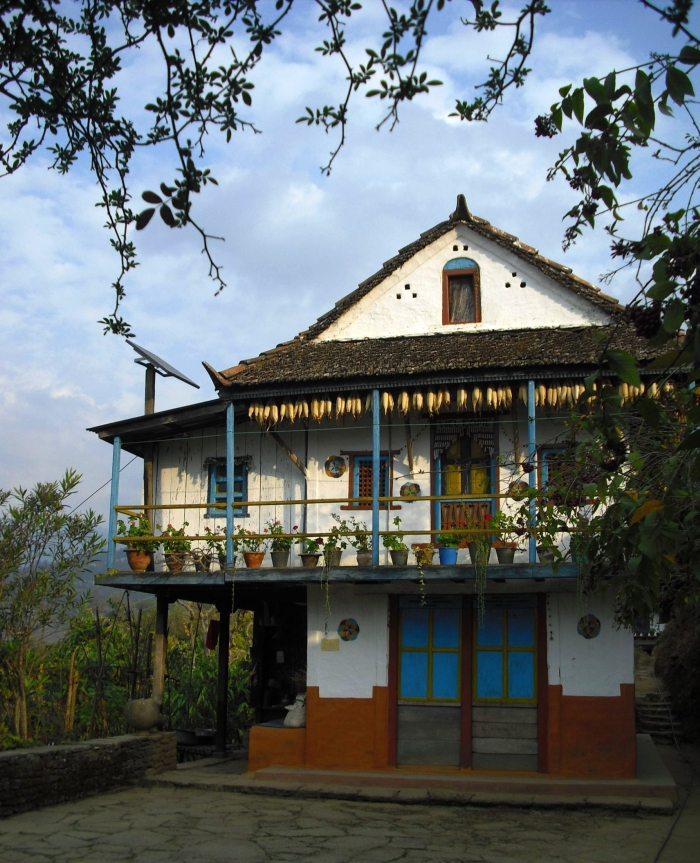
\includegraphics[height=8cm]{figures/house.jpg}
\caption{A Yakkha house in Tumok village}\label{house}
\end{figure}


The Yakkha have a rich tradition of processing bamboo (\emph{phabu}). Bamboo products are abundant in all aspects  of material culture, from house construction to manufacturing various kinds of sieves, baskets and the most delicate and tiny purses, combs and needles, as shown in \figref{phabu}.

Another craft is weaving mats from straw and maize leaves. Furthermore, fabrics and shawls are produced on looms.  The pattern found on traditional Yakkha shawls (\emph{phopma}) is shown in \figref{phopma}. 


 \begin{figure}[h]
 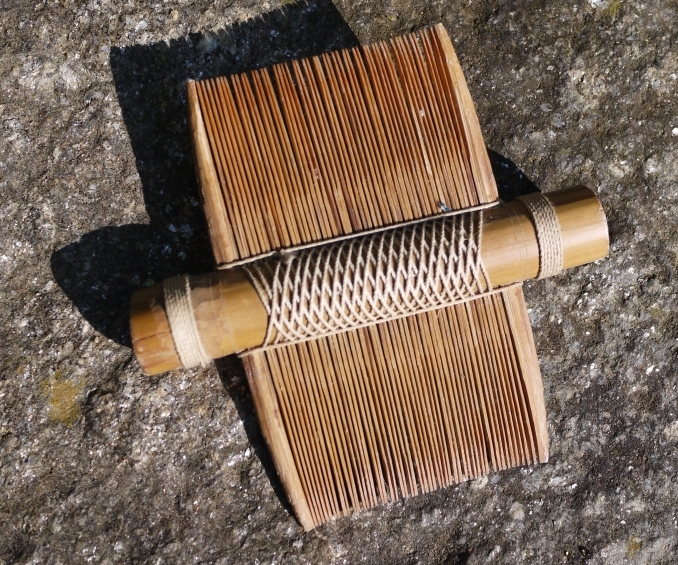
\includegraphics[width=0.30\textwidth]{figures/comb.jpg}
 \hfill
 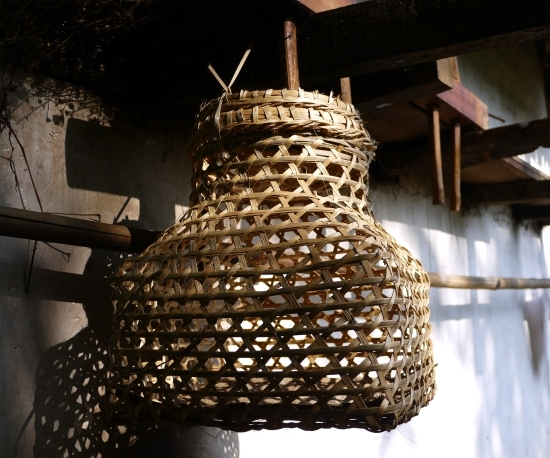
\includegraphics[width=0.30\textwidth]{figures/kangyong.jpg}
 \hfill
 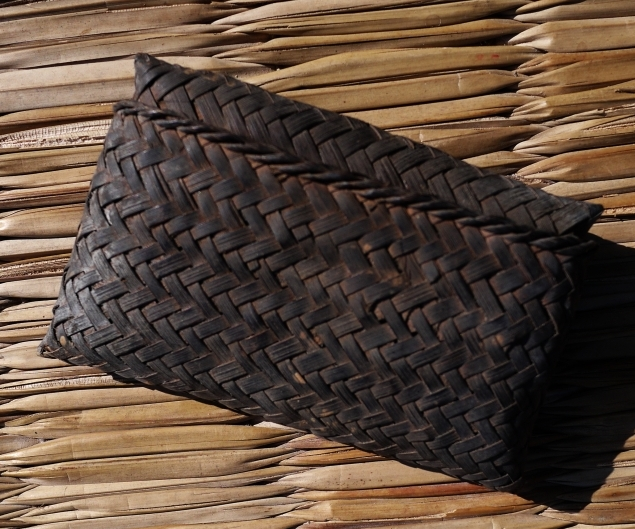
\includegraphics[width=0.30\textwidth]{figures/phepi.jpg}
 \caption{Bamboo  products: \emph{sigikma} \rede{comb}, \emph{kaŋyoŋ} \rede{chicken basket}, \emph{phepi} \rede{purse}}\label{phabu}
 \end{figure}



\begin{figure}[h]
\centering
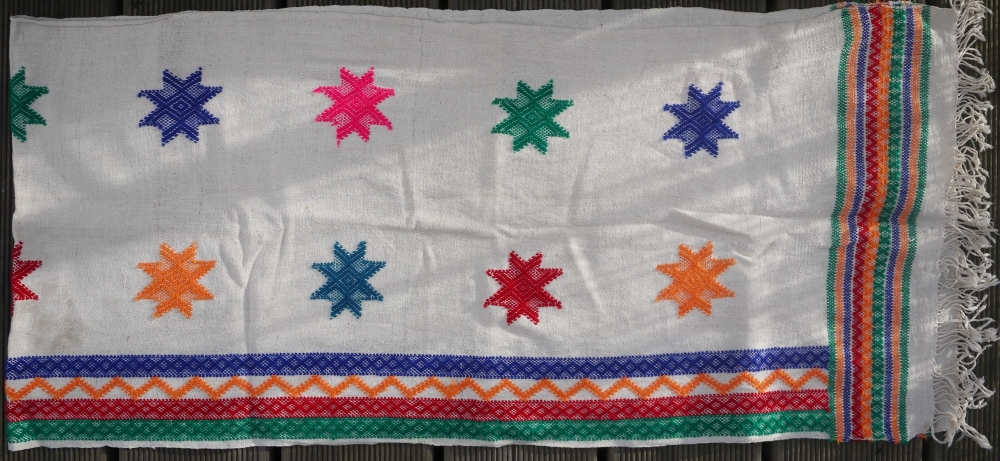
\includegraphics[height=4cm]{figures/phopma.jpg}
\caption{Yakkha \emph{phopma} (shawl)}\label{phopma}
\end{figure}

\subsubsection{Social organization and religion}\label{social}

The Yakkha religious sphere and social organization are shaped by the pan-Kiranti tradition that is called \emph{munthum} in Yakkha, in which the ancestors play a major role. The term \emph{munthum} also refers to a body of orally transmitted texts in which the deeds and journeys of the ancestors come alive. \citet{Gaenszle_Redefining} notes that, despite differences in ritual systems and practices, this ancestral tradition is shared by  all Kiranti groups. The \emph{munthum}

\begin{quote}
[...] comprises histories of the origin of the ancestors, beginning with the primal creation of the universe and the emergence of natural and cultural orders and continuing to the settlement of the ancestral territory. It also concerns the proper means of communicating with ancestors and ritually maintaining the order they have established. The term, then, has an additional meaning: it evokes a way of life predefined by the ancestors, a self-enclosed world rooted in the past. \citep[224]{Gaenszle2000Origins}
\end{quote}

The social order, but also the physical and mental health of individuals, is ultimately related to the ancestors. This is also illustrated by rituals such as \emph{saya pokma} (literal translation: \rede{raising the head soul}), which is known in Yakkha and in other Kiranti groups. It is undertaken to re-unite individuals, whose well-being is endangered, with the primaeval ancestral order. In her anthropological-psychological study on Lohorung culture, for example, \citet{Hardman2000_Other} notes that the main frame of reference in that culture is one in which

\begin{quote}
... the \rede{natural} ancestral order [...], as recorded in their myths, has to be constantly recreated and the unity between nature, the superhuman, and the human reaffirmed. Failure to do this would lead to depression, increased sickness, possibly death, and ensuing chaos. In contrast, repetition of ancestral worlds and adherence to ancestral order acts like recharging the cosmos. It brings vitality. \citep[12--3]{Hardman2000_Other}
\end{quote}

For  Yakkha people, the ancestral order is equally important. A key feature of this order is the division of the Yakkha society into clans (called \emph{choŋ}), which is critical not only in marriage restrictions but also in the ritual sphere. \citet[201]{Russell1992_Yakha} notes the following clan names in Yakkha (square brackets indicate his transcriptions where deviating from the orthography used in this work): \emph{Linkha}, \emph{Chala} [challa], \emph{Koyoŋwa} [koyoŋa], \emph{Khamyahaŋ} [kammieŋ], \emph{Limbukhim} [limbuhim], \emph{Hoŋhoŋba}, \emph{Koŋgren}, \emph{Choŋgren}, \emph{Maʔkruk}, \emph{Yaʔyukhim}, \emph{Taʔyum}, \emph{Pubaŋgu}, \emph{Oktubaŋ}, \emph{Somyeŋ}, \emph{Khayakhim} [khayakim], \emph{Heŋwa}, \emph{Ilumbaŋ}, \emph{Tiksalaŋ}, \emph{Thampara}, \emph{Ibahaŋ}, \emph{Yuwahaŋ}. I further recorded the clan names \emph{Elaba}, \emph{Hangsewa} and \emph{Huture} in mythical narratives. 

Apart from these clans, there are is another concept called \emph{sametliŋ} \rede{spiritual clan}. There are different  \emph{sametliŋs} for the women and for the men of each clan. Women of one clan may, however, share their spiritual clan with men of another clan. In contrast to clan  (\emph{choŋ}) affinity, the \emph{sametliŋ} of a woman does not change after marriage. The \emph{sametliŋs} outside one's family are not widely known, in contrast to a person's \emph{choŋ}. They are only significant in dealing with spirits (\emph{cyaŋ}) \citep[166]{Russell1992_Yakha}.

Personal names (mostly Indo-Aryan nowadays), are not widely used. It is rather common to adress a person by the respective kinship term, or by a teknonym \rede{X's father} or \rede{X's mother}. 

The ritual specialists responsible for holding the ancestral rituals are called \emph{Maŋgaŋba} in Yakkha. They undertake rituals for each household on occasions like births, marriages and deaths. The task of the \emph{Maŋgaŋbas} is to maintain the ancestral order and good relations with the spirit world (there are several potentially dangerous spirits such as \emph{soghek} - ghosts of people who have died an unnatural death). Other religious practitioners are \emph{chamwas},  \emph{bijuwas} (a Rai term), \emph{phedaŋbas} (a Limbu term), \emph{dhamis} (a Nepali term), but I cannot offer a typology of their features and their tasks. Jointly celebrated festivals (above the clan level or even above the village level) are \emph{casowa} (Nepali: \emph{udhauli}) in late autumn and \emph{yuchyaŋ} (Nepali \emph{ubhauli}) in spring \citep[102ff.]{Kongren2007Indigenous}.\footnote{In his ethnological study, \citet{Russell1992_Yakha}  does not mention these festivals, so their names as well as  celebrating them this way might be a relatively new development.} On these occasions and also on marriages, people gather in a circle and dance a complicated choreography slowly to the sound of huge drums beaten by some men in the circle (\emph{keilakma} \rede{dancing the drum dance}). \todo{Please do not use \emph{ff.}. Please give full page ranges}

The Yakkha society is patrilineal and patrilocal. With regard to marriages, it is important to note that there are two distinct steps taken to incorporate the bride into the clan of her husband. The actual marriage is only the first step, called \emph{mandata}. The second step is called \emph{bagdata}, and is undertaken years, sometimes decades, after the marriage. In the \emph{bagdata}, the husband has to ask his in-laws for their daughter again, and only after this ritual does she become a member of his clan. If the wife dies before the \emph{bagdata} has been asked for, her natal home will undertake the death rites for her.

 
\section{Genealogical affiliation}\label{genetic}

Yakkha is a Sino-Tibetan language, belonging to the Greater Eastern branch of Kiranti, a group of Tibeto-Burman languages spoken in Eastern Nepal.\footnote{Although not  undisputed, it is assumed by many scholars that Sino-Tibetan can be divided into a Sinitic and a Tibeto-Burman branch, the latter containing at least 300 languages \citep{Bradley1997_Tibeto-Burman, Matisoff2003Handbook}.}  Beyond this basic classification, the question of how to group Kiranti languages with other Sino-Tibetan languages is still a controversial issue, as in general, subgrouping in the large and incredibly diverse Sino-Tibetan language family has proven to be rather difficult (see e.g. \citealt[Chapter 3]{Hyslop2011_Kurtop} for an overview of the different models of reconstruction that have been proposed).

\citet{Shafer1974_Introduction} identified Kiranti (which he called East Himalayish) as a sub-branch of Bodic, together with three further branches: Bodish (including Tibetan and Tamangic languages), West Himalayish and West Central Himalayish (including Magar and Chepang). Similarly, \citet{Bradley1997_Tibeto-Burman} suggested that the Kiranti languages, together with Magaric and Newaric languages, form the sub-branch Himalayish. 

A different view is entertained by \citet{LaPolla2003_Overview},  who includes Kiranti in a group he calls Rung (including, most importantly, the rGyalrongic languages, the Dulong languages, the Kiranti languages,  Kham, and the West Himalayan languages Kinauri and Almora), on the basis of shared person marking morphology and a reflexive/middle suffix \emph{*-si} (except for rGyalrong).  What makes any classification even harder is that not even the question of the antiquity of person marking in Tibeto-Burman has been settled yet (see e.g \citet{DeLancey2010_Towards, Jacques2012_Agreement} who argue that such a system can be reconstructed, and \citet{LaPolla2001_Role, LaPolla2012_Comments}, who argues that agreement marking systems in Tibeto-Burman languages are independent innovations).

Kiranti languages can be grouped into a Western and a Central-Eastern branch (with a Central and a Greater Eastern sub-branch), as shown in \figref{fig-Kiranti-tree} (\citealt{Bickeletal_Firstperson}). Central-Eastern Kiranti is characterized by a loss of voiced initials by merging voiceless and voiced initials \citep{Michailovsky1994Manner}. Voiced stops with phonemic value rarely occur, though voiced allophones are possible, as a result of post-nasal and intervocalic voicing, for instance in Yakkha and in Athpare \citep[505]{Ebert2003Kiranti}. 

\todo{Maybe a TikZ-picture would be better suited here than qtree using node and child node. Right now, this tree is hardly readable and I would like to enlarge it. However I have not found a way to manually set vertical distances in qtree which is necessary here in order to scale this tree correctly. I think tikZ can do this. }

	\begin{figure}[h]
	\resizebox{\textwidth}{!}{
		\setlength{\qtreepadding}{2pt}
		\setlength{\abovecaptionskip}{10pt}

		{\scriptsize
		\Tree 
		[.\fbox{\textbf{Kiranti} }
			[
				[.{Western\\(*ʔC → C)} 
				{Chaurasiya\\(*ch → s):\\Jero\\Wambule} 
				{Northwestern:\\Bahing/Bayung\\Hayu\\Sunuwar/Koĩc} 
				{Upper Dūḍhkośī:\\Khaling\\Dumi} 
				] 
				[.{Midwestern\\(*ʔp,*ʔt → b,d):\\Thulung\\Koyu}
				] !\qsetw{-2cm}
			]
			[.{\fbox{\textbf{Central-Eastern}}\\(*voiced → voiceless;\\*ʔk,*ʔc → kh, ch)} 
				[.{Central\\(*ʔp,*ʔt → b,d)} 
					{Khambu\\(*ʀ→ g, hr):\\Kulung\\Nachiring\\Sampang\\Sam} 
					{Southern:\\Camling\\Bantawa\\?Dungmali\\Puma} 
				] 
				[.{\fbox{\textbf{Greater Eastern}}\\ (*ʔp,*ʔt → ph, th)} 
					{Upper Aruṇ\\(PE *ph,*th → $\emptyset$):\\Lohorung\\Yamphu\\Mewahang}  
					!\qsetw{1cm} [.{Eastern\\(ʀ,r → y)} 
						{\fbox{\textbf{Greater Yakkha}}:\\\fbox{\textbf{Yakkha}}\\?Mugali\\Ch\textbari l\textbari ng\\Chintang\\Athpare\\Belhare (PE *th → $\emptyset$)} 
						{Limbu\\(ch → s)} 
					] 
				] 
			] 
		]
		}
	}
	\caption{Kiranti subgrouping, according to \cite{Bickel2008Seminar}}\label{fig-Kiranti-tree}
	\end{figure}
	
 
Yakkha undoubtedly belongs to the Greater Eastern branch. A distinctive feature of Greater Eastern Kiranti languages is the change of pre-glottalized stops into aspirated stops  (or zero, in the case of /*ʔt/, see further below):  */ʔts/ > /tsʰ/, */ʔp/ > /ph/,  */ʔk/ > /kh/ (see \tabref{soundchange} for comparative data).\footnote{The table is based on data from \citet{Driem1993A-grammar, Driem1987A-grammar, Bickeletal2009Puma, Kongren2007Yakkha} and my own data.} The Greater Eastern branch splits into Upper Arun (Lohorung, Yamphu and Mewahang) and Eastern Kiranti, to which Yakkha belongs. Eastern Kiranti is characterized by  the change of  initial */r/ and */R/ into /y/ \citep{Driem1990The-fall}.

Within Eastern Kiranti there are two groups, which are the various Limbu dialects on the one hand and the so-called Greater Yakkha group, with Chintang, Belhare, Athpare,  Chɨlɨng and Yakkha, on the other hand. Some languages of the Greater Yakkha branch are characterized by the loss of the aspirated coronal stop, compare e.g. Limbu \emph{thuŋ} \rede{drink} with Yakkha (and Belhare) \emph{uŋ} \citep{Bickel1997Dictionary}. Furthermore, the aspirated affricate /tsʰ/ (see above) has undergone a further change to /s/ in Limbu, compare e.g. Limbu \emph{sarumma} with Yakkha \emph{chalumma} \rede{second-born girl} (for further examples see \tabref{soundchange}). 

Rhotic consonants, although they do  not occur word-initially  in Yakkha, are found word-internally. The claim made by  \citet{Driem1990The-fall} that [l] and [r] have a complementary distribution and are thus allophones in Eastern Kiranti cannot be confirmed for Yakkha: both sounds occur in similar environments word-internally  (cf.  \tabref{r-l} on page \pageref{r-l}), and no environment was found  in which [l] and [r] show allophonic variation  in Yakkha  (see also \sectref{rhotic}). Thus, although finding “proper” minimal pairs for /l/ and /r/ is difficult, /r/ is a phoneme in Yakkha.

\begin{table}[t]
{\small
\begin{tabular}{llllll}
\lsptoprule
{\sc Proto-}&  {\sc Dumi}  &  	{\sc Puma} &  {\sc Yakkha} &  {\sc Limbu} &  \\
 {\sc Kiranti }  &   ({\sc western}) &  ({\sc central}) &  ({\sc eastern}) &   ({\sc eastern}) &{\sc gloss} \\
\midrule
\char"002A /d/		& 	deːn	&  		ten 		&  	ten	&  tɛn	& 	\rede{village}	 \\
\char"002A /j/		& 	ju&  ca&  ca &  ca&  \rede{eat}	 \\
\char"002A /b/		& 	bhiʔi&  pooŋ&  pik &  pit & 	 \rede{cow} \\
\char"002A /r/		&  rep	&  rep &  ep&  yep & 	  \rede{stand}\\
\char"002A /r/		&  roʔdi	&  roduŋ&  yakthuŋ&  yak & 	  \rede{Kiranti} (autonym)\\
\char"002A /R/		&  r\textbari m	&  rum&  yum&  yum& 	 \rede{salt} \\
\char"002A /ch/		&   	&  chapd-&  chep & sap   & 	 \rede{write} \\
\char"002A /ʔc/		&  	&  chakd &  chekt &  sak& 	 \rede{close} \\
\char"002A /ʔp/		&  puŋ	&  buŋ &  phuŋ &  phuŋ& 	 \rede{flower} \\
\char"002A /ʔt/		& 	t\textbari ŋ&  duŋ&  uŋ&  thuŋ& 	 \rede{drink} \\
\char"002A /ʔt/		& 	&  dok &  ak & thak & 	 \rede{loom} \\
\lspbottomrule
\end{tabular}
}
\caption{Examples of Kiranti sound correspondences}\label{soundchange}

\end{table}

Based on a comparison of the verbal person marking paradigm, the closest re\-lative of Yakkha within the Greater Yakkha branch is Belhare. The two languages exclusively share the following markers: a suffix \emph{-ka \ti -ga} indexing second person arguments (any role), and an underspecified nasal prefix \emph{N-} indexing third person plural S and A (3>2.{\sc sg} and 3pl>3) in Yakkha, and  3nsg.S and 3>2 in Belhare \citep[551]{Bickel2003Belhare}. 



\section{Sociolinguistic context}\label{socioling}
\subsection{Dialectal variation}\label{sc-dialect}

The variety documented here is spoken in Tumok village and surrounding areas, e.g. in Salle. No detailed dialectal study has been undertaken for Yakkha yet. Based on phonological differences and distinct exclamative words, I tentatively propose three further dialects: one spoken in the area around Ankhinbhuin (Angbura, Hombong, Phakling), one spoken in the area around Dandagaun and one spoken towards the north, in Kingring and Kharang villages. 

\tabref{dialects} illustrates dialectal differences. The Kharang dialect is different from the other dialects, for instance, in having a second person possessive marker \emph{i-} instead of the unspecified nasal prefix that is found elsewhere,  and in having a clause-final exclamative particle \emph{ikhok}. Apart from this, I do not have data on this dialect. 

Yakkha has a general phonological rule of voicing consonants in post-nasal and intervocalic position. The rule has different domains of application across the dialects: in Tumok and in Dandagaun it does not apply to aspirated consonants, while in Ankhinbhuin it applies to both aspirated and unaspirated consonants. Furthermore, I noticed that in Dandagaun,  /o/ gets raised to /u/, at least in some lexemes. In the Tumok  dialect, the person marker for first person acting on second is \emph{-nen}, while in the Ankhinbhuin dialect it is \emph{-nan} (cf. also the data from Omruwa (Angbura) in \citealt{Driem1994The-Yakkha}). In Dandagaun and Ankhinbhuin honorific imperative forms calqued upon Nepali are used, while in  this is not common in Tumok. I have no data on the varieties spoken in the south of the Dhankuta district, in the village of Namsaling in Ilam district and in India.


\begin{table}
\centering
\begin{tabular}{lllll}
\lsptoprule
{\sc tumok}	&	{\sc dandagaun}	&{\sc ankhinbhuin}	&	{\sc kharang}&	{\sc gloss}\\
\midrule
\emph{mma}	&\emph{mma}	&\emph{mma}	&\emph{ima}		&\rede{your mother}\\
\emph{nniŋga}	&\emph{nniŋga}	&\emph{nniŋga}		&	\emph{iniŋga}	&\rede{your}\\
\emph{i \ti ina \ti iha}	&\emph{i \ti ina \ti iha}&\emph{i \ti ina \ti iha}		&	\emph{iruk}	&\rede{what}\\
\emph{cokma}&\emph{cukma}	&\emph{cokma}			&	(no data)	&\rede{do, make}\\	
\emph{ŋkhya(ci)}&\emph{ŋkhya(ci)}&\emph{ŋghya(ci)}&		(no data)	&\rede{they went}\\	
\emph{mphopma}&\emph{mphopma}	&\emph{mbhopma}			&	(no data)	&\rede{your shawl}\\
\emph{piʔnenna}	&\emph{piʔnenna}	&\emph{piʔnanna}	&	(no data)	&	\rede{I gave it to you}\\
\emph{coeba}	&\emph{cama leŋniba}	&\emph{cama leŋniba}&	(no data)	&\rede{Please eat.}\\
\emph{haʔlo}	&	(no data)	&\emph{khoʔo \ti kho}&\emph{ikhok}&(exclamative particle)\\
\emph{=pa}	&			\emph{=pa}	&\emph{=aŋ}&	(no data) &(emphatic particle)\\
\lspbottomrule
\end{tabular}
\caption{Dialectal variation within the Yakkha region}\label{dialects}
\end{table}



In Marek \textsc{vdc} in Dhankuta (Marek, Ghorlikharka, Jitpur, Andrung, Magwa, Saldang villages),  a variety is spoken that is so different from the other Yakkha varieties (as perceived by  the speakers of Yakkha, too) that it cannot be called a dialect of Yakkha any more. The linguistic differences notwithstanding, the speakers are perceived as belonging to the Yakkha group on ethnic grounds. The language is called Lumba-Yakkha in the Ethnologue (ISO 639-3: luu).\footnote{\citet{Levisetal2015_Ethnologue}, http://www.ethnologue.com, accessed on Dec. 20 2013} I have not heard this designation in Tumok, the language was usually referred to as \emph{māreki bhāsā} (Nepali; \rede{the language from Marek}). The Marek variety has, for instance, undergone the sound change from /ch/ to /s/ that is also known from Limbu. Crucially, the pronominal paradigm and the verbal inflection are different from Yakkha, for instance the second person prefix \emph{a-}  (otherwise known from Athpare and Chintang, see \citealt{Ebert1997A-grammar, Bickeletal2007Free}) instead of the Yakkha suffix \emph{-ka}. \tabref{lumba} provides some exemplary data collected in 2010 with a speaker from Marek, but no detailed study has been undertaken yet. 

\begin{table}
\centering
\begin{tabular}{lll}
\lsptoprule
{\sc marek}&	{\sc tumok}	&		{\sc gloss}\\
\midrule
\emph{hoʔli}&\emph{imin}&\rede{how}\\
\emph{pisa}&\emph{picha}&\rede{child}\\
\emph{seŋma}&\emph{chimma}&\rede{to ask}\\
\emph{hima}&\emph{i \ti ina \ti iha}&\rede{what}\\
\emph{mahuma}&\emph{maghyam}&\rede{old woman}\\
\emph{pahuba}&\emph{paghyam}&\rede{old man}\\
\emph{nhandi}&\emph{khaʔla}&\rede{like this}\\
\emph{aŋga}&\emph{ka}&\rede{I}\\
\emph{aŋciŋ}&\emph{kanciŋ}&\rede{we} (du)\\
\emph{aŋniŋ}&\emph{kaniŋ}&\rede{we} (pl)\\
\emph{ŋkhan}&\emph{nda}&\rede{you} (sg)\\
\emph{habe}&\emph{heʔne}&\rede{where}\\
\emph{hannalam}&\emph{heʔnhaŋ}&\rede{where from}\\
\emph{akhaʔneʔna}&\emph{khemekana}&\rede{you go}\\
\emph{=na}&\emph{=na}&(nominalizer)\\
\emph{-ma}&\emph{-ma}&(infinitive marker)\\
\lspbottomrule
\end{tabular}
\caption{Marek data in comparison with Tumok data}\label{lumba}
\end{table}

\subsection{Endangerment}\label{endangerment}

According to the Nepali census of 2001 \citep{\textsc{cbs}2001Report} and the UNESCO Working Paper No. 7 \citep{Toba2005Unesco}  there are 14,648 native speakers out of about 17,000 ethnic Yakkha. The number of native speakers makes up 0.06 per cent of the Nepalese population. This census, however, seems highly optimistic to me, since Yakkha is barely spoken in half of the Yakkha area, and even where it is spoken the youngest generation (below 20 years of age) does not commonly use Yakkha, even though they might have a passive command of the language. Specific domains such as ritual, mythological and traditional ecological knowledge are known only by a few (usually) elderly people. I did not find any monolingual Yakkha speakers; all speakers are at least bilingual with Nepali,\footnote{The official language in Nepal is the Indo-Aryan language Nepali. It is used in official communication,  in commerce and in  education. Since the constitution of 1990 which followed the first \emph{Jana Andolan} (People's uprising), all languages spoken as mother tongues in Nepal are considered national languages, which grants the speakers the right to be educated in their mother tongue \citep{Turin2007_Diversity}. This is, however, hard to implement, given that more than 100 languages are spoken in the country.} and proficiency in other neighbouring languages such as Bantawa and Limbu is also common.

One reason why Yakkha  speakers shift to Nepali is the already mentioned migration outward for economic and educational reasons, but there are also whole  villages inside the  homeland that have switched to Nepali. For instance, while Yakkha is still vividly spoken in Tumok, it is difficult to find speakers in the neighbouring villages Mamling, Waleng and in the old garrison town Chainpur (a former center for trade in the region). Most speakers of Yakkha are found in the south of the Yakkha region.

A well-known reason for this development is the low prestige that indigenous languages have long  had compared to Nepali. Since the creation of the Nepali nation state in the eighteenth century under the rule of King Pr̥thvī Nārāyaṇ Śāha (1723–1775), Nepali has been propagated as the national language, and people have  not been encouraged to speak other languages. Much damage was also done under the Panchayat System (1961–1990), where the use of indigenous languages was actively discouraged under the policy of “One Nation, One Language” \citep[20]{Toba2005Unesco}.

Language shift is complex and can be understood on both macro and interactional levels of analysis. In the Yakkha region, education beyond the primary school level is available exclusively in Nepali or English.\footnote{This is also reflected in the negative correlation between the educational level and the number of Yakkha students. According to the 2001 census, the number of Yakkha students beyond the primary level was 6915, the number of those who have passed \textsc{s.l.c} was 878 and the number of those with a degree was 89 in 2001 \citep{\textsc{cbs}2001Report}.} At the primary level, Yakkha language classes have been introduced in a number of schools recently (starting in 2009), but Yakkha is not the medium of instruction in other subjects. Yakkha people are not represented in the government beyond village level \citep{\textsc{cbs}2001Report}. Even in the villages, official posts in education and administration are still overwhelmingly held by people from  non-indigenous backgrounds, simply because there are not enough Yakkha people who could work in these positions. This social and economic bias exerts additional pressure on the speakers of Yakkha, and these dynamics are one of the reasons why Yakkha-speaking parents use Nepali with their kids. 


Another factor destabilizing the language situation are marriages with people outside one's  own linguistic community, for instance Yakkha-Limbu marriages. Generally, bilingual or multilingual families are of course not problematic, to the contrary, multilingualism is rather the norm world-wide (see \citealt{Turin2007_Diversity}). But with the additional pressure that comes from Nepali, children from multilingual families nowadays often grow up with Nepali as the only language they speak fluently. 

These developments cannot simply be related to a lack of interest in the parents to pass on their language. According to my own observations, the tendency not to speak Yakkha is even present in the children of those people who have a high ethnic awareness and who are engaged in a number of activities towards preserving their language and culture. The tension between preserving one's  ethnic and linguistic heritage and participating in modern society is well-known in theoretical approaches to language loss, but it is nevertheless hard to resolve for the affected individuals.

In the past decades, with multi-party democracy having started in 1990, and even more so in the post-monarchy era that has followed the civil war (1996–2006) and the second \emph{Jana Andolan} (People's Uprising) in 2006, activities aiming at the preservation of the indigenous languages and cultures have increased. In the case of Yakkha, for instance, the Kirant Yakkha Chumma (Indigenous Peoples Yakkha Organization) have implemented Yakkha lessons in a few primary schools in the Yakkha region.  School books have been completed up to class five already, with the plan to reach class eight. Dictionaries, literary works and even songs and music videos have been created lately by members of the community who feel the urge to do something before it is too late (cf. \sectref{earlier-work}). The long-term impact of this welcome development remains to be seen. To properly assess the endangerment of a language, an in-depth study in its own right would be necessary. The loss of Yakkha in a wide geographic area and in the youngest generation are, however, very clear and alarming signs.





